\documentclass[12pt,a4paper]{report}
\usepackage{color}
\usepackage{amsmath}
\usepackage{graphicx}
\usepackage{upquote}
\newcommand{\blank}[1]{\hspace*{#1}}
\usepackage{setspace}
%\onehalfspacing
\doublespacing
\newcommand*{\rom}[1]{\expandafter\@slowromancap\romannumeral #1@}
\makeatother
\usepackage{fancyhdr}




    \pagestyle{fancy}
\usepackage{blindtext}

\lhead{\footnotesize{Bitcoin: A Peer-to-Peer Electronic Cash System}}
\chead{}
\rhead{}
\lfoot{\footnotesize{Department of ECE, PESIT-BSC }}
\cfoot{}
\rfoot{Page \thepage}
\renewcommand{\headrulewidth}{1pt}
\renewcommand{\footrulewidth}{1pt}
%\footnotetext{Department of ECE, PESIT-BSC  \blank{6cm}}




\usepackage
[
        a4paper,% other options: a3paper, a5paper, etc
        left=1.25in,
        right=1in,
        top=0.75in,
        bottom=0.75in,
        % use vmargin=2cm to make vertical margins equal to 2cm.
        % us  hmargin=3cm to make horizontal margins equal to 3cm.
        % use margin=3cm to make all margins  equal to 3cm.
]
{geometry}
\usepackage{lipsum}
\usepackage{multirow}
\pagenumbering{roman}
\usepackage{pgf}
\usepackage{pgfpages}
\pgfpagesdeclarelayout{boxed}
{
  \edef\pgfpageoptionborder{0pt}
}
{
  \pgfpagesphysicalpageoptions
  {%
    logical pages=1,%
  }
  \pgfpageslogicalpageoptions{1}
  {
    border code=\pgfsetlinewidth{2pt}\pgfstroke,%
    border shrink=\pgfpageoptionborder,%
    resized width=.95\pgfphysicalwidth,%
    resized height=.95\pgfphysicalheight,%
    center=\pgfpoint{.5\pgfphysicalwidth}{.5\pgfphysicalheight}%
  }%
}
\pgfpagesuselayout{boxed}

\begin{document}
\begin{titlepage}
\begin{center}
\vspace{3cm}
\textup{\begin{LARGE}{\textbf {TECHNICAL SEMINAR REPORT}}\end{LARGE}}\\[10.0cm]

\begin{LARGE}{\textbf {THE BITCOIN NETWORK AND PROTOCOL}}\end{LARGE}\\[7.0cm]

\vfill
\begin{flushright}


\begin{LARGE} \textbf{SAWAN SINGH MAHARA}\\\textbf{1PE14EC128}\\\end{LARGE}
\vfill
\end{flushright}

\end{center}
\end{titlepage}

%\setcounter{page}{i}
\begin{center}\underline{ \Large\textbf{ACKNOWLEDGEMENT}}\end{center}
It is always a pleasure to remind the faculty of PESIT-BSC for their sincere guidance and support to intensify my wisdom and give me the opportunity to present what I have learned. I would like to thank to my parents for the encouragement, enthusiasm and invaluable lessons given, which have ingrained in me a sense of curiosity and wonder to attain an unquenchable thirst for knowledge. Without this, I would not have been able to complete this undertaking adequately.\\

I would like to accredit \textbf{Dr. J Surya Prasad} Director/Principal of PESIT BSC for the sterling facilities and resources that were made freely available to me which has enabled me to successfully complete this research and presentation venture.\\

Furthermore, my gratitude to \textbf{Prof. Chiranjeevi} would not go overlooked, and I am grateful for his tremendous support and advice, without which, none of this would have materialised.\\

Finally, my appreciation goes out to the project coordinators, \textbf{ Mrs.Vidya T V},\textbf{ Mr.Shivaraj J Karki}, and \textbf{ Mr. K Rama Murthy}, the Assistant Professors in \textbf{The Department of Electronics and Communication} for spearheading and organising the seminar discussion for the academic year  \textbf{2018}.
I also apologise to all the other unnamed who have helped me in various ways to have successfully complete this endeavour.

\newpage
\begin{center}\underline{ \Large \textbf{ABSTRACT}}\end{center}
\vspace{5mm}
 \begin{flushleft}
 A peer-to-peer payment scheme over the internet, using electronic cash is usually mediated by a third party, for example, a financial institution. This obligation makes way to some issues which this report addresses. Bitcoin achieves decentralisation by being distributed and forgoing the need of any kind of trust between performing parties. The bypass for the need of external validation from a third party is done by employing cryptography and hashing. All this while managing to be be Byzantine Fault Tolerant. The aim of this study is to expose the underlying working principles of the Bitcoin  network and protocol which would, in effect, lead to a clearer picture of cryptocurrencies and blockchain technology, as a whole.
 \vspace{5mm}
  
 Digital signatures are used for validating payments originating from a peer while hashing is used to ensure permanent data integrity. The double-spending problem is also mitigated by clever use of the blockchain proof-of-work aspect, which would be further dealt with in this report. To maintain only a single record of all transactions, which would enable verification of transactions simpler, the longest chain of blocks would be considered as the only source of everything that has occurred on the network. This implementation of this largest chain is such that it would have only come from the largest pool of CPU power.
  \vspace{5mm}
  
 The Bitcoin network is reliable, secure and safe, as long as the majority of the CPU power is controlled by nodes that are non-hostile to the network. Meeting this requirement, the Bitcoin system ensures that attackers would be unable to generate the longest chain, thus keeping all transaction records that ever occurred unaltered even in the slightest form. Setting up the network is not resource intensive and so, the distributed nature of the system would have its evolution and reach, unhindered. This feature allows for nodes to freely leave and rejoin the network as well.
 \vspace{10mm} 
 
%\vspace{15mm}
%\textbf{Categories and Subject Descriptions: Image Processing}
%\vspace{5mm}
%\textbf{Key words: Distinct Invariant Features, Affine Distortion}
%\vfill

\newpage

\begin{center}\Large\textbf{TABLE OF CONTENTS}\end{center}
\vspace{10mm}

\begin{tabular}{|c |l| c|}\hline
\textbf{CHAPTER} & DESCRIPTION\blank{7cm} & \textbf{Page no.}\\ \hline
1 & Inroduction & 1\\ \hline
2 & History &3\\ \hline
3 & Motives and Benefits & 5\\ \hline
3.1 &  The Reasons For Bitcoin &5\\ \hline
3.2 &  The Benefits of Bitcoin & 6\\ \hline
4 &  Digital Currency & 8\\ \hline
4.1 &  Unauthorised Removal of Funds & 8\\ \hline
4.2 & Repeat Transactions & 10\\ \hline
4.3 & Double Spending & 10 \\ \hline
5 & Proof of Work & 12\\ \hline
5.1 & The 51\% Majority & 12\\ \hline
5.2 & The Counter-Intuitive Solution & 13\\ \hline
6 & Key Concepts & 17\\ \hline

6.1 & Hashing & 17 \\ \hline
6.2 & Merkle Trees & 19 \\ \hline
7 & The Block Chain & 21 \\ \hline
7.1 & The Block & 21 \\ \hline
7.2 & Mining & 23 \\ \hline
7.3 & Transactions & 24 \\ \hline
8 & The Caveats & 27 \\ \hline
9 & Conclusion & 29 \\ \hline
10 & References & 30 \\ \hline
\end{tabular}

\newpage

\begin{center}\Large\textbf{LIST OF FIGURES}\end{center}

\vspace{10mm}

\begin{tabular}{|c |l| c|}\hline
\textbf{FIGURE} &  DESCRIPTION\blank{7cm} & \textbf{Page no.}\\ \hline
1 &  Graphical illustration of a the block chain  & 2 \\ \hline
2 & The price of Bitcoin in USD, over the years & 4\\ \hline
3 &  Brief Overview of Digital Signature Verification   & 10\\ \hline
4 &  The Double Spending Issue & 12\\ \hline
5 &  Fork Attack  & 14\\ \hline
6 &  Pre-Processing and Initialisation in SHA-256    & 19\\ \hline
7 &  SHA-256 Core Logic        &20\\ \hline
8 &   Merkle Root Structure    &21\\ \hline
9 &  A Block with its Various Fields   & 23\\ \hline
10 &  The Sensitivity to the Inputs of Hashing Functions  & 24\\ \hline
11 &  Multiple Input and Multiple Output Transaction Structure  & 26\\ \hline
\end{tabular}
\newpage
\pagenumbering{arabic}
\setcounter{page}{1}

\begin{center}\underline{  \Large\textbf{CHAPTER1}}\end{center}
\begin{center}\underline{ \Large \textbf{INTRODUCTION}}\end{center}
\vspace{10mm} 
Bitcoin is a currency that allows for peer-to-peer transactions over the internet which is not regulated or owned by a single institution. It was introduced in 2009 by a pseudo-anonymous person(s) by the name Satoshi Nakamoto as an open source software.
\vspace{10mm}
It is synonymous with cryptocurrency as it employs cryptographic principles to ensure authenticity of all transactions that occur with it. As it is not owned by a single institution, say a bank or even associated with any country, the US Treasury has declared Bitcoin as a decentralised currency. This was the first of its kind and its existence has solved a few major problems that would be inherent in using currency which is stored as a sequence of bits on a computer.
The bitcoin network works by using a string of attached, publicly accessible ledgers which is called a \textbf{blockchain}. Each ledger is simply named as a \textbf{block} and it contains transactions and other information necessary to locate, number and verify it. Transactions are always broadcast to the entire network to make sure that it can be validated. All information about a block can be condensed into a hash and this is called the block hash. This blockchain can be thought of as a linked list data structure wherein the pointers to the linked list are replaced by a block header.

\begin{figure}[h]
\centering
\caption{Graphical illustration of a the block chain}
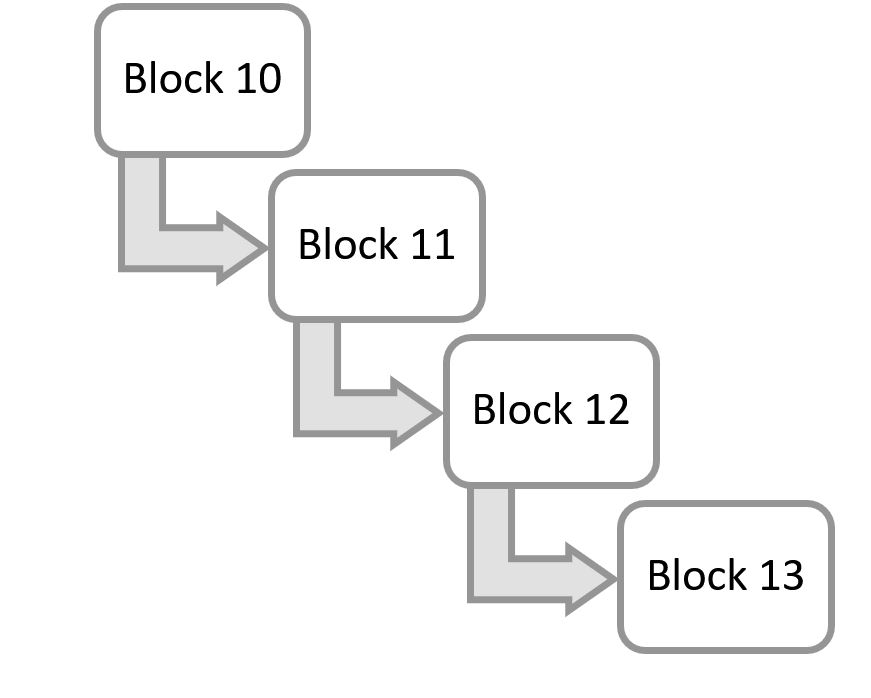
\includegraphics[scale=0.4]{pics/Block.JPG}

\end{figure}

\vspace{10mm}

To grow this chain, a block has to be added to its end. The latest one added would contain the latest transactions that have occurred using this cryptocurrency. Nodes which add a block to the blockchain would have to prove that it has done \textbf{work} by solving a hashing puzzle, which on completion would yield that node the \textbf{transaction fees} as well as a default base pay, in bitcoins. This base pay introduces new bitcoins into the network and is the only source of generation of these coins, barring the first initial block, termed as the \textbf{genesis block}.
\vspace{10mm}
Bitcoins can be obtained in exchange for other currencies, products, and services. or users can buy, send, and receive bitcoins electronically for a nominal fee using wallet software on their a personal computer, mobile device, or a web application.
Thus it can be used as a full fledged medium of monetary exchange between individuals. Since no country owns it, it is resilient to the economic conditions of many countries around the globe.

\newpage
\begin{center}\underline{  \Large\textbf{CHAPTER2}}\end{center}
\begin{center}\underline{ \Large \textbf{HISTORY}}\end{center}


\vspace{10mm}
In 2008, a paper surfaced on the internet by an anonymous Satoshi Nakamoto, which people believe can be accredited to the 2008 US financial crisis. An exploit to create many bitcoins did occur in 2009, which was promptly fixed and was the last known major fault in this system till date. Bitcoin's worth in physical currency has been fluctuating since its inception and has since gone numerous cycles of appreciation and depreciation.
Due to this, it has been thought of by some as the next gold revolution, and by others, nothing more than just a bubble of inflation which could burst anytime.
\vspace{5mm}

In 2013, bitcoin found use in transactions over some mainstream websites. WordPress started in November 2012 followed by OKCupid in April 2013, for example.
With the sudden popularity of this currency, its value rose as more and more people wanted to trade with it and in 2013, for the first time, it crossed USD 1000 and never came back down, ever since. The year 2017 saw its price rise to 5000, and then in November that year, all the way to USD 18000. It did fall in the coming months and has been hovering around the USD 10000 mark.


\begin{figure}[h]
\centering
\caption{The price of Bitcoin in USD, over the years}
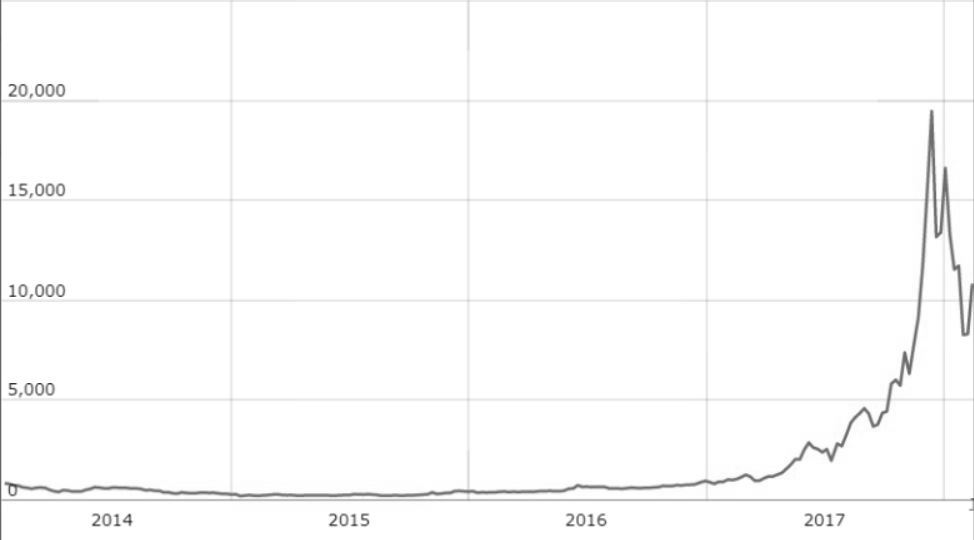
\includegraphics[scale=0.4]{pics/Price.JPG}
\end{figure}

\vspace{10mm}
Being open source, the community has grown exponentially since 2009 with many developers working on Bitcoin and ways to improve it. As its founder Satoshi Nakamoto has been anonymous ever since, some people have raised concerns over this system, many linked to the open source nature of this cryptocurrency many.

As the source code and implementation is open and freely available, anyone can participate in this decentralised system. And just as how like current developers do not control or regulate bitcoin, even its founder Satoshi had no influence over it since its inception.

\newpage
 
\begin{center}\underline{  \Large\textbf{CHAPTER 3}}\end{center}
\begin{center}\underline{ \Large \textbf{MOTIVES AND BENEFITS}}\end{center}

\vspace{10mm}
\textbf{3.1 THE REASONS FOR BITCOIN}
\vspace{10mm}

As discussed earlier, the 2008 financial crisis was one of the leading reasons for the creation of the bitcoin. 
To summarise, the financial crisis of 2008 in the US was caused by banks which lent out risky loans to attract new customers, which would enable banks to get money to give more loans and so on. This was like a bubble, and eventually it burst in 2008. As the loans were risky, many banks were not paid back and the list of loan defaulters gradually increased. This made many banks collapse and file for bankruptcy. In addition to giving out risky loans, these banks also used people’s money to invest in various opportunities, which didn't work as intended, causing a further downfall.
\vspace{10mm}
People had trusted these banks to keep money safe, but in turn they lost it all. Noticing this widespread bankruptcy, the American Government tried saving these banks. They attempted a bail out by repaying people's money. These funds came from the taxes that were payed and it caused an overall fall in the development of the nation.
Here lies the first problem. Financial institutions do not keep people's money idly sitting. It is used to lend loans and offer other services, which could lead to a collapse like this.
Another widespread issue is that when governments overspend and are out of funds, they request banks to print more money, which in turn just devalues the currency as more of it is available.
\vspace{10mm}

Bitcoin solves these issues by account of it being a decentralised financial system. Nobody owns or regulates the money, and every transaction is accounted for.  These coins either are spent, or stay put. Not moving anywhere.

\newpage
\vspace{10mm}
\textbf{3.2 The Benefits of Bitcoin}
\vspace{10mm}

By decentralising and distributing the monetary powers of a financial institution, bitcoin can leverage consensus to make decisions. This means that nobody would tend to make risky decisions and that leads to some interesting implications, such as:

\begin{itemize}

 \item \textbf{Fewer risks} \newline People buying things using Bitcoin need not share too much information about themselves like their bank account details, names or addresses. This is a desirable aspect as people are vulnerable to attacks if their identity and bank statements are known. \newline 
 The latter isn't too hard  to obtain, if the attacker is willing enough.
 Sellers of goods and services are also benefited as these transactions are secure, irreversible, and only work if the customer has enough funds in the first place, leading to no such thing as cheque bounces. This also protects merchants from losses occurring via fraud or fraudulent chargebacks.
  
  \vspace{10mm}
  \item \textbf{Payment freedom} \newline
  As Bitcoin ensures that the maximum funds that go out of an address is available in the first place, people could buy anything at any price, without worrying too much about processing time and checks that happen in banks. Also since the internet is up and running 24/7 people are allowed to pay anytime, anywhere, not looking out for things like bank holidays. No borders. No imposed limits. Bitcoin enables its users to be in full control of their money.
  \vspace{10mm}

 \item \textbf{Transparency and neutrality} \newline 
 Every single bitcoin and fractional values of it are freely available to account for and see for any an everyone, in real time. As anybody can view it, even people who do not participate in bitcoin transactions can do this too. Rest assured that the identities of the transacting parties would never be known.\newline
 Neutrality is ensured as no individual or organisation can control or manipulate the Bitcoin protocol because as it is cryptographically secure. This allows the core of Bitcoin to be trusted for being completely neutral, transparent and predictable.
 
  \vspace{10mm}
 
  
  \item \textbf{Low fees} \newline 
  Currently, there are zero transaction fees, if the user isn't in an imminent situation to have their transaction verified. Users include fees with transactions if they want to receive priority processing, resulting in faster confirmation of transactions. This allows for a market of merchant processors to assist in processing transactions by converting bitcoins to fiat currency and depositing funds directly into merchants' bank accounts daily. As these services are based on Bitcoin, they can be offered for much lower fees than with PayPal or credit card networks
  
  \vspace{10mm}
  
  \item \textbf{Control and Security} \newline 
  The only person authorised to move money out of an address is the one who holds the account information only. Thus, any merchant has no way to to force unwanted or unnoticed charges, which is common practise in today's institutional banking services. This offers strong protection against identity theft. Also, if desired, Bitcoin users can also protect their money with backup and encryption.
  

\end{itemize}


\newpage

\begin{center}\underline{  \Large\textbf{CHAPTER 4}}\end{center}
\begin{center}\underline{ \Large \textbf{Digital Currency}}\end{center}

\vspace{10mm}

To fully appreciate the development of the Bitcoin protocol, it would be desirable to look at the inherent difficulties that one would face, if they attempt to build such a system on their own. Starting from the most fundamental issues and then building up on it, we can understand why the protocol does what it does.
As it was earlier established that the bitcoin network works as a series of ledgers, and that it is open source, so anyone can add or remove names, it leads us to the first issue.
\vspace{10mm}

\textbf{4.1 UNAUTHORISED REMOVAL OF FUNDS}
\vspace{10mm}

Simply put, anyone that makes a transaction, would have their wallet address in the transaction. An attacker could just use this address and take out more funds from this account. Let us call this a \textbf{type 1 attack}. \newline

This is where digital signatures come into play. Simply put, a digital signature is a variant of asymmetric encryption. In such an encryption technique, an individual is given a \textbf{private key} which is a set of 256 or more, bits of information. This key is to be known only to them, and nobody else. With this, one is capable of doing two things. 
\begin{itemize}
    \item Construct any number of shareable \textbf{public keys}. This is similar to the private key in the sense that it's also a string of characters. It differs from its counterpart in the sense that everyone is allowed to view it. The property of this key is that it can decrypt anything that is encrypted by the private key, which leads us to the other use of the key.
    \item Private or public keys can encrypt data using an encryption algorithm and are extremely secure. Also, anything encrypted by a private key can only be decrypted with a public key and vice-versa.
\end{itemize}
The second aspect of the private/public key pair is useful in digitally signing documents. Since it is established that only the possessor of a public key can decrypt a message scrambled by a private key, encrypting a message with such a key for the purpose of secrecy is redundant. \newline
However, it can be used to verify if the possessor of the private key had in fact, encrypted that particular message. This is because if any other key was used to encrypt data, the public key would fail to work and thus, a person's identity can be verified.
This is exactly why digital signatures are used to verify transactions occurring.
An attacker would have to know the private key of a person, to validate transactions on their behalf, which is very hard to do if the said person is very secretive about their private key.

\begin{figure}[h]
\centering
\caption{Brief Overview of Digital Signature Verification}
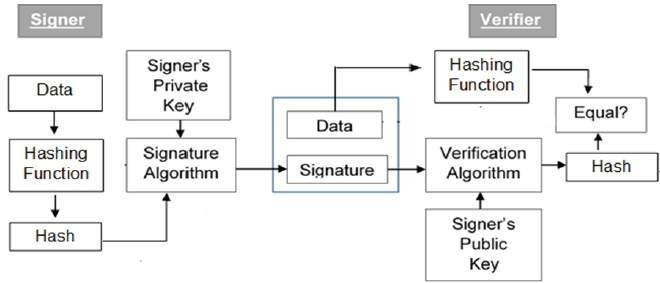
\includegraphics[scale=0.6]{pics/model_digital_signature.jpg}
\end{figure}
\vspace{10mm}

As shown above, the sender's signed data is hashed. A hashing function just takes an input set of characters of a a variable length and puts out, always, a fixed length of characters which appear random but are just pseudo-random. This means that if the same set of input were to be inputted again, it would result in the same hash. Hasing will be further looked into, later on.
\newpage
\textbf{4.2 REPEAT TRANSACTIONS}
\vspace{10mm}

Digital signatures solve the problem of unauthorised transaction validation by a third party. An issue still imminent, however, is that the attacker could be the person who is receiving the verified funds themselves. Here, they could simply copy the same transaction multiple times on the ledger. This would work since the transaction was initially verified in the first place. \newline
This can be easily circumvented, however, by the use of serial numbers in every transaction. Since all digitally signed transactions are hashed, every successive transaction, even with the same amount, would appear different on the ledger.\newline

The need for serial numbers indicates that a third party must be present to issue and validate these serial numbers. A bank, of some kind. This is true and the bitcoin does have a \textit{third party} to issue and validate these transactions. This third part is not a financial institution or a singe large entity, as is the case with ordinary currency. This is done by other nodes of the network itself.

\vspace{10mm}
\textbf{4.3 DOUBLE SPENDING}
\vspace{10mm}

Other nodes in the network issue a consensus on whether or not a transaction is valid. Only then will a recipient of funds accept the payment. This type of a system is good and safeguards the sender from fraud. However, the fraudster could be the sender themselves. They can exploit one simple fact that the recipient of funds are the only the ones verifying transactions. The other nodes do not check if these funds were used elsewhere, just that if that particular serial number is correct.\newline

The sender of bitcoins could just pay two or multiple people, the same transaction coin, just with a different \textbf{to} address. This issue is called the double spending.
When the network realises that the same coin is being spent twice, it drops the last coin added, thinking that it is a type 1 attack when it was not so.
\vspace{10mm}
\begin{figure}[h]
\centering
\caption{The Double Spending Issue}
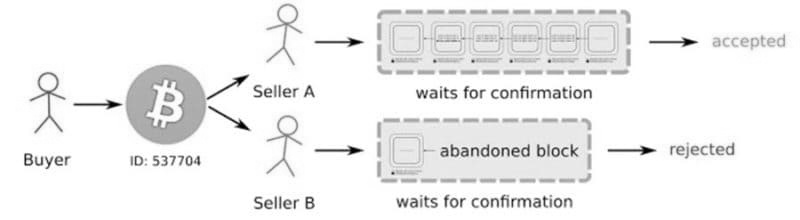
\includegraphics[scale=0.5]{pics/double_spending.jpg}
\end{figure}
\vspace{10mm}

Circumventing this is rather easy to do. The issue lay in the fact that only the ones receiving funds were verifying it.By allowing other nodes to fully \textit{hear} these transactions, we can mitigate the double spending problem. This is because everyone on the network cannot be fooled by the sender as they can easily see that the same coin is being spent twice or more. Thus, the network can choose the drop both transactions, and it would never work.\newline
This is exactly why the bitcoin network broadcasts every detail of a transaction. The network can not only verify if \textit{serial numbers}, but also verify that each coin is being spent only once.

\newpage
\begin{center}\underline{  \Large\textbf{CHAPTER 5}}\end{center}
\begin{center}\underline{ \Large \textbf{PROOF OF WORK}}\end{center}
\vspace{10mm}

\textbf{5.1 THE 51\% MAJORITY}
\vspace{10mm}

The previous chapter dealt with issues like double spending and repeat transactions. These were mitigated without a third party like a financial institution by utilising consensus as its replacement. This would work to prevent small scale attacks from crippling the network.\newline
If an attacker is determined, however, they can exploit the network's heavy dependency on consensus. This can be done by realising that the majority say comes from computers, not people. More specifically, computer programs. An attacker can very well create multiple instances of nodes and then pretend to verify all transactions coming from their account. 
\vspace{10mm}

The recipient of funds would not know that the consensus was achieved by one individual as it would appear as if it had come from multiple nodes. This problem arose because anyone on the network could verify transactions. The need for trust was still in place. A trust that all the consenting parties were in fact for the good of the network, and not out to exploit it.\newline
Thus, to successfully cripple this currency scheme, one has to simply have enough resources to create instances that are 51\% or more than the currently existing nodes on the network.\newline
An attacker could also \textit{fork} the blockchain, listening to transactions and verify them independently. They would then have control over what type of transactions go on there as well. This is not good as then one entity would be in control of the chain. Herein lies the issue. They could simply rewrite the history of transactions then. By doing this, one could potentially get back funds payed for some goods or services and use it elsewhere in effect to the merchants giving everything for free.
\newline

\vspace{10mm}
\begin{figure}[h]
\centering
\caption{Fork Attack}
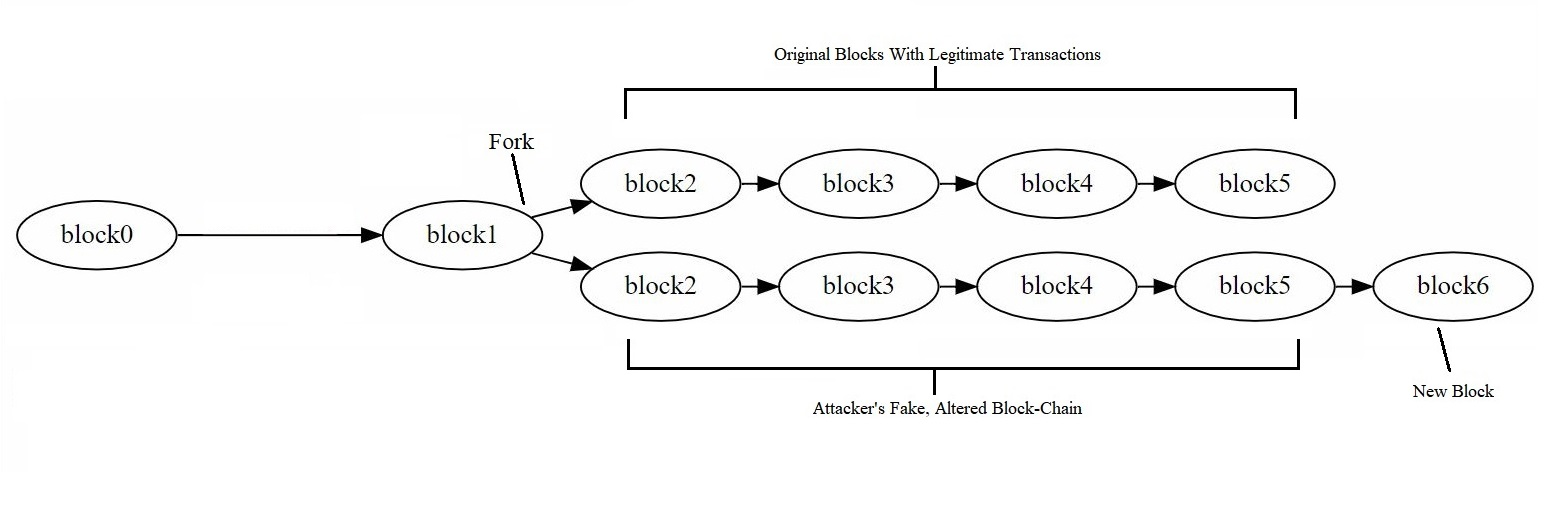
\includegraphics[scale=0.4]{pics/fork.jpg}
\end{figure}


\vspace{10mm}
\vspace{10mm}
\textbf{5.2 THE COUNTER-INTUITIVE SOULUTION}
\vspace{10mm}

If it was made sure that there is only one block chain that the entire network could follow and refer to, then the network would be a secure and trustable source of record. To do this, the network gives out bitcoins to every node that that verifies transactions and add them to the blockchain. \newline
This seemingly counter-Intuitive solution has a catch, however. Every addition to the block can only be done by nodes that have the most \textbf{computational power}. This is so that an attacker that intends to modify the blockchain, must not only possess the 51\% majority, but also must ensure that all those 51\% nodes are the most powerful systems on the network. The second condition is very hard to meet and practically unfeasible, if the bitcoin network were to be populated by cooperative nodes. \newline

\vspace{10mm}
To understand why this system is safe, let us assume that a dishonest sender \textit{S} of funds requests for a service from a merchant \textit{M} who would then create a public key for this transaction and sends it as the address to which the payment has to be made. Now, \textit{M} waits until the transaction is confirmed and a few blocks, say \textbf{z} in number are linked after it, in the blockchain.\newline

In this original chain, \textit{S} has paid \textit{M}. Parallelly, if \textit{S} were to create a fraudulent block, without that transaction having ever taken place, to add it back to the chain and fool \textit{M}, \textit{S} would have to rebuild \textit{z} blocks as well, and also any other blocks that would have arrived by the time they were replicating the \textit{z+1} blocks. \textit{M} may be alerted when that happens, but the \textit{S} hopes it will be too late.\newline

What we will now show is that if it is made hard to put in a single block on the blockchain network, so hard that if someone attempts to fork the chain anywhere, it should be highly unlikely that they succeed to fool anybody unless and until they own 51\% or more of the entire \textit{capability to put blocks on the chain} or simply put, that much computational power so that they win the consensus. Let us assume that\newline

\textit{p} = the probability an honest node makes the next block\newline
\textit{q} = the probability the attacker makes the next block\newline
\textit{$q_z$} = the probability the attacker will ever catch up from \textit{z} blocks behind\newline
Then, it can be shown that \newline
\begin{equation*} 
  q_z = \begin{cases}
 1  & \text{if $p \leq q$} \\
 $$\left(\dfrac{q}{p}\right)^z$$ & \text{if $p > q$}
\end{cases}
\label{eqn:simple_one} 
\end{equation*}
\newline
And if we model the time taken by an attacker to succeed as an ergodic Poisson process with average $\lambda$, we can conclude that 

\begin{equation*} 
  \lambda = z\frac{q}{p}
\end{equation*}
\newline

Now to get the probability the attacker could still catch up to \textit{z} blocks and  surpass it to fool \textit{M}, we multiply the Poisson density for each amount of progress he could have made by the probability he could catch up from that point. Doing this would give us the probability of his success as:

\begin{equation*} 
 %1-\sum_{k=0}^{z} \dfrac{\lambda^(k)e^(-\lambda)}{k!}
P\left( k \right) =1-\sum_{k=0}^{z} \frac{{e^{ - \lambda } \lambda ^k }}{{k!}}\Bigg(1-\left(\dfrac{q}{p}\right)^{(z-k)}\Bigg)

\end{equation*}

This concludes that if the attacker must create more than \textit{z} blocks, they must create $k>z$ number of them and then the probability of that happening, and \textit{S} succeeding dies down exponentially when this is attempted, since it would take some significantly finite amount of time for the attacker to not only catch up to, but also surpass \textit{z} blocks. 
\vspace{10mm}

Thus, the bitcoin network migrates the need for trust in the consenting parties, to the need for a hope that there is no attacker with the computing power of 51\% or more. This is not an unreasonable requirement if the network is widespread enough. Then there would always be cooperative nodes as it would be more economical to try and get transactions verified in return for the reward by the network than to just try and attack it.
\vspace{10mm}

The network is said now said to be Byzantine Fault Tolerant. This means that it mitigates the Byzantine Faults in distributed networks. A Fault of such a kind is an inherent limitation in a system, where information propagation from one component to another would never be a 100\% accurate. There would always be a non-zero probability that the information is false. Proof-of-Work makes the Bitcoin network Byzantine fault Tolerant as only nodes with a lot of computational power can propogate information.
\vspace{10mm}

Since it is now hard to put a block on the blockchain, a node wouldn't just add one transaction at a time it would instead listen to many transactions happening, put them all in a block and then try to add that block onto the blockchain. The network caps the total size of the block so that it easy to handle and move around.
\newline
The more transactions a block has the, larger it gets in size and so if it fails to be confirmed, all those transactions would be lost. To prevent this from happening often, the Bitcoin protocol has a block size limit to enable speedy propagation and reduce anomalies. Each block thus has a size limit of 1,000,000 bytes.

\newpage


\begin{center}\underline{ \Large \textbf{CHAPTER 6}}\end{center}
\begin{center}\underline{ \Large \textbf{KEY CONCEPTS}}\end{center}
\vspace{10mm}

\textbf{6.1 HASHING}


As explained earlier, adding a block onto the blockchain is made hard. To understand how hard, we must look into what the core idea behind hashing really is. Simply put, hashing is a set of rules that ensures that data of any length is scrambled into one fixed length of characters. This scrambling is done to appear random, but is not at all so. A hashing logic ensures that if the same input were fed to it again, the exact same sequence of random characters are put out again.
\vspace{10mm}

There are many hashing algorithms out there, but bitcoin employs one named SHA-256, which stands for \textit{Secure Hashing Algorthim-256}. Fully explaining this algorithm is not a task that this report intends to undertake, but an attempt to give a vague sense of its intricacy would be made, however.
\vspace{10mm}
The output of SHA-256 is 32 characters long, but the ideal input to it would be 64 characters. If the input is too small, appropriate number of zeros would be padded to it. If it is too large, then it would be split into chunks of 64 characters, and each chunk would undergo SHA-256 separately to give out 32 characters. Then, 2 sets of these 32 characters would be combined into 64 characters and SHA-256 would be run on it again. This is repeated until there is only one 32 character output left.

\vspace{10mm}

Let us try hashing a 160 character string. This would be divided as three groups of size 64, 64 and 32 characters each. The SHA-256 would first take one set of 64 characters, and group 4 of them together for a total of 16 groups. Then another 17th group is made from a linear combination of a few of the already present groups, adding up a constant from a given source. Now that the 17th group is made, a similar thing is repeated all the way until 64 groups are made. \newline

\vspace{10mm}

Now, as the output is fixed to 32 characters, 8 groups of these are initialised to some values, given by the NSA. In the next iteration, the state B is made as the old A, C to B and so on, excepting the new states of the groups A and E. A is made as a linear combination of a few of the old states, with some constant that is given by the NSA and the first group of the initial message, namely Group 1. Let's call this as X. Similarly, E is also constructed that way, adding Group 1 to it as well. Let's denote this as Y. \newline

\vspace{10mm}
\begin{figure}[h]
\centering
\caption{Pre-Processing and Initialisation in SHA-256}
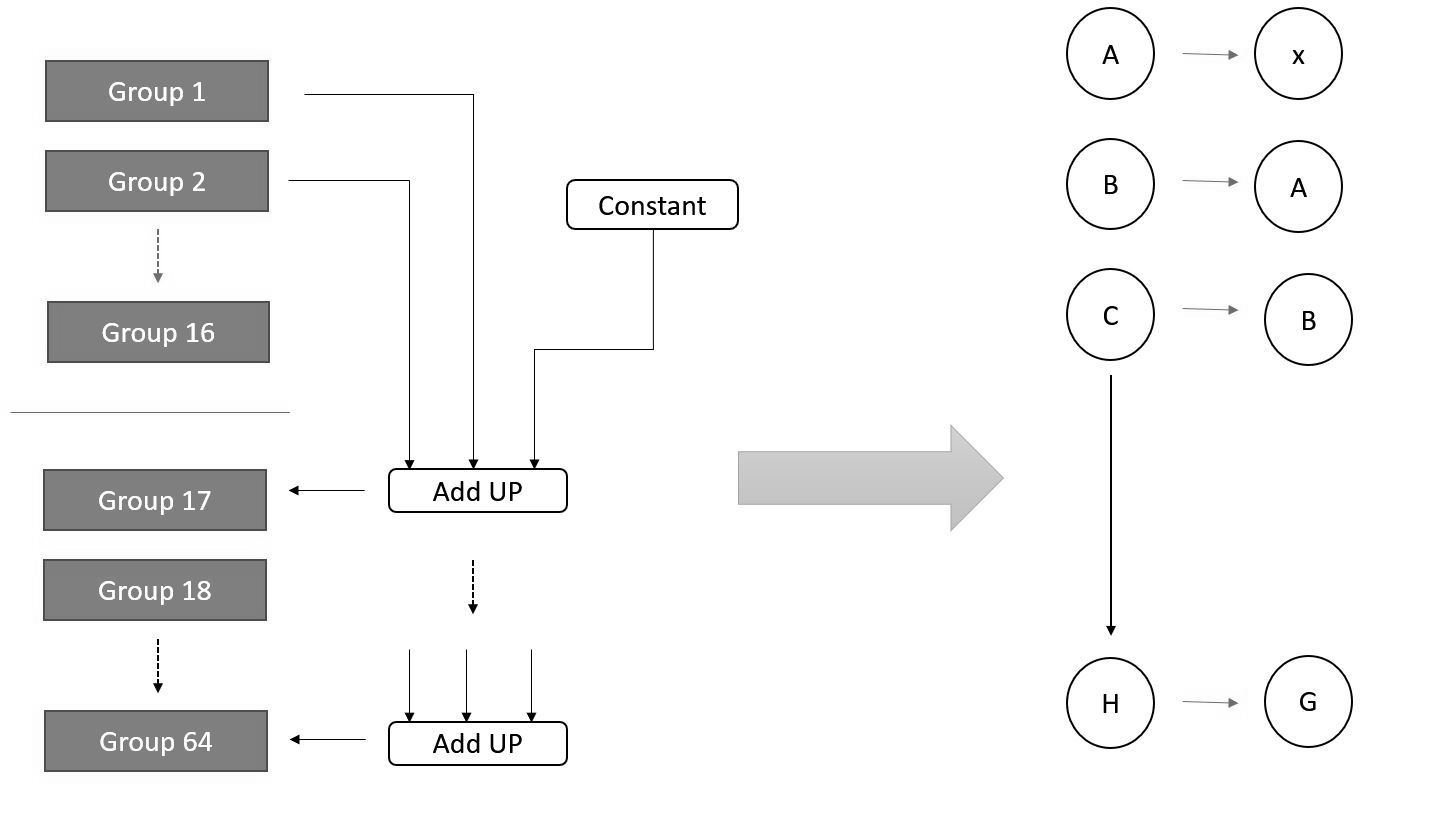
\includegraphics[scale=0.25]{pics/sh256.JPG}
\end{figure}
\vspace{10mm}



X's and Y's are computed 64 times, exhausting all the 64 groups of the message, by repeating the process mentioned above. The final step would be to add this output to the initial values A through H. This would be parse one.\newline
Now the initial message was 160 characters long, the hash of only the first 64 character long group was made. This algorithm would be repeated for the second 64 character long group, the only difference being that the initialisation of A's through H's would not be from the NSA, but the hash of the first 64 characters. After this is done, the final hash is computed on the last remaining 32 bits by concatenating it with the output of the second SHA-256 parse.\newline
This output would finally be the hash of the 160 character message taken earlier. 

\vspace{10mm}
\newpage
The reason SHA-256 is computed, is because of the sheer number of intricate steps involved make it very sensitive to the input message. This means tha event a single bit flip in the message would result in a completely different hash. \newline
Not only that, but also the fact that the algorithm is heavily dependant on the message, to reach a particular state, implies that the only way to get a desirable hash, would be to just keep guessing different inputs multiple times and hope for the best. The reason why one would do this would be explained later.


\vspace{10mm}
\begin{figure}[h]
\centering
\caption{SHA-256 Core Logic}
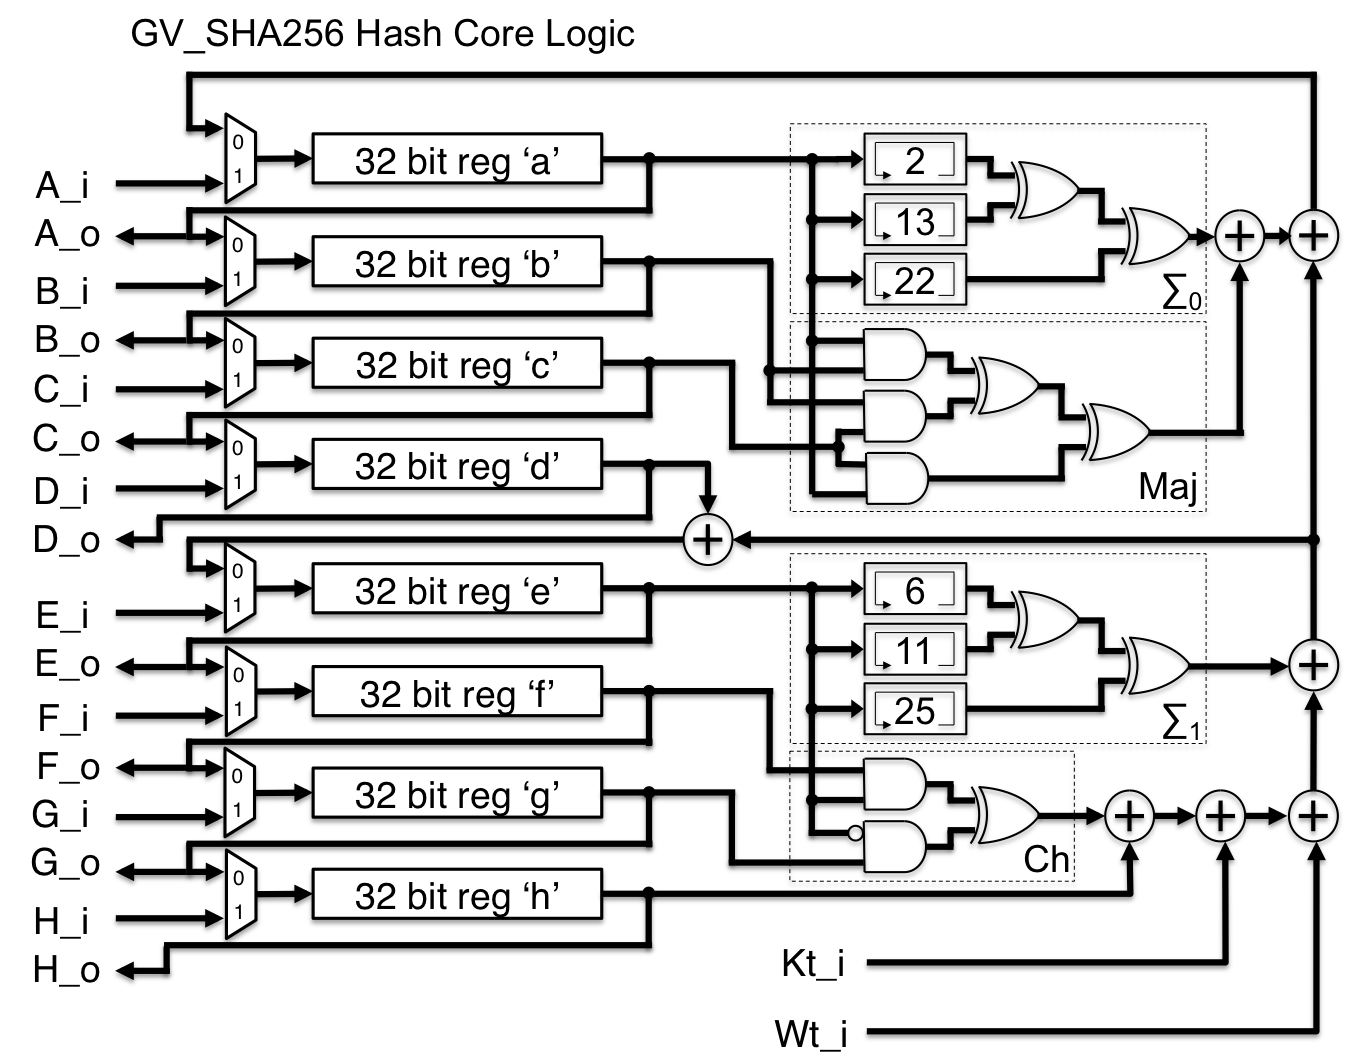
\includegraphics[scale=0.50]{pics/usercontent,img,1471445681.png}
\end{figure}
\vspace{10mm}

\textbf{6.2 MERKLE TREES}
\vspace{10mm}

A prerequisite to understanding how hard it is to alter transactions in a block on the blockchain would be through Merkle Trees. This is a structure which is implemented on the bitcoin network to accomplish two things.
\begin{itemize}
    \item Speed up the hashing of the block. Why this would be done is explained soon.
    \item Have a method to quickly verify transactions, by omitting redundant checks.
\end{itemize}
\newpage
\vspace{10mm}

A Merkle root was found to be the perfect answer to these two requirements. It is simply a series of hashes, starting from the raw data. Data is first hashed in groups of two's and the result of that hash is hashed with the result of another group of two. This is repeated until there is one final hash left. This hash that's left is called a Merkle root. In bitcoin, transactions are hashed to obtain the Merkle root of all the transactions. This one 32 character long string represents all the transactions in that block, and so is independent of the number of transactions that are recorded on the block since it is always a fixed length string of characters.\newline

\vspace{10mm}
\begin{figure}[h]
\centering
\caption{Merkle Root Structure}
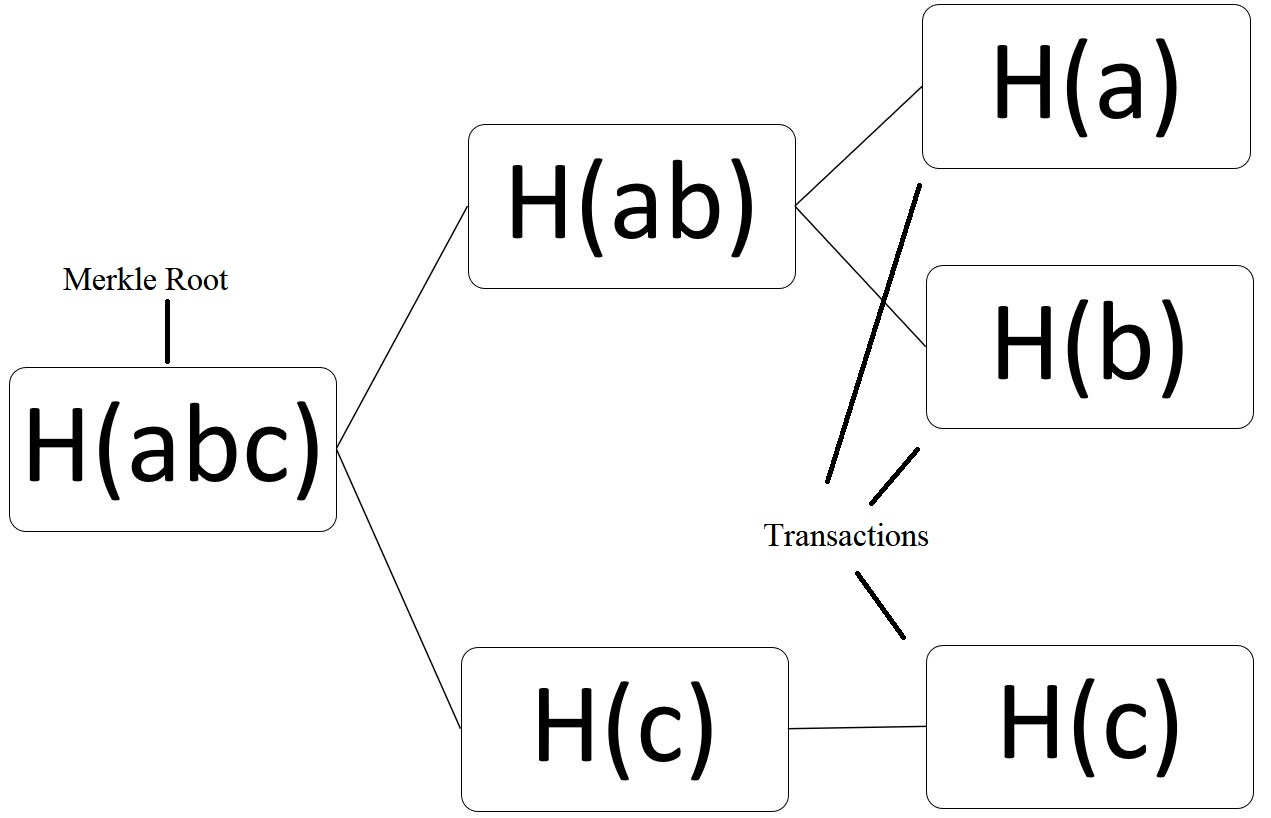
\includegraphics[scale=0.4]{pics/Merkle.JPG}
\end{figure}
\vspace{10mm}
\newline
This merkle root thus can be a very great way of condensing all the transactions into one single fixed length hash. If any of the transactions are altered, the root would obviously change as the tree has a hash as the inputs in higher levels. This tree, also serves as a way to verify transactions, by just traversing through one branch, instead of all branches.

\newpage


\begin{center}\underline{ \Large \textbf{CHAPTER 7}}\end{center}
\begin{center}\underline{ \Large \textbf{THE BLOCKCHAIN}}\end{center}
\vspace{10mm}
\textbf{7.1 THE BLOCK}
\vspace{10mm}

The block has been so far referenced as just holding transactions. This is true, but the block holds more than just transactions. It has a body, that holds the raw transactions, which on their own have a unique structure. Blocks also have a block header, which contains the following fields.
\begin{itemize}
    \item \textbf{Version number}\newline
    This is an addition to help distinguish the two actually running forks of bitcoin.
    Although theoretically it was intended to have only one single blockchain, it had to be forked practically due to the block size limitation of 1MB. The second version of bitcoin has the capability of holding a larger number of transactions.
    \item \textbf{Previous Block Hash}\newline
    A block's hash is nothing but the header field of the block, hashed. This field in the block header contains the hash of the previous block. The only exception to this rule is the \textit{genesis block}, which is the very first block on the blockchain.
    \item \textbf{Merkle Root}\newline
    The Merkle root, as discussed earlier, can be thought of as the fixed length signature of all transactions that are going on the block.
    \item \textbf{Time Stamp}\newline
    The rough time at which the block is being verified, is put on here.
    \item \textbf{Bits}\newline
    This an encoded version of the targeted \textit{difficulty} of the block. This is something used to ascertain that the block was verified by a computationally strong node.
    \item \textbf{Nonce}\newline
    A random guess that is used by nodes to allow it to add their block onto the blockchain.
    
\end{itemize}

The last two fields, namely the Nonce and the Bits are somethings that weren't spoken about earlier. These are fields used in ascertaining that the node that put the particular block on the blockchain, actually had done a lot of work. The \textit{proof} in Proof-of-Work, so to speak. The process of getting a block onto the blockchain, after verifying the transactions collected, is termed as \textbf{Mining.}

\vspace{10mm}
\begin{figure}[h]
\centering
\caption{A Block with its Various Fields}
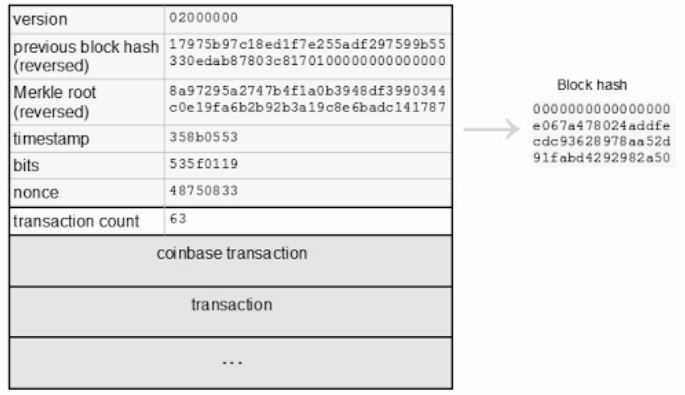
\includegraphics[scale=0.7]{pics/blk.JPG}
\end{figure}
\vspace{10mm}



\vspace{10mm}
\newpage

\vspace{10mm}
\textbf{7.2 MINING}
\vspace{10mm}

As ascertained earlier, the hash of any given string of characters are seemingly random and involve a series of intricate steps that make it almost impossible to predict the outcome of the hashing algorithm, for any given input. This fact is exploited in making a \textit{Proof-of-Work} for the system. The bitcoin mining process can be summarised as follows.


\vspace{10mm}
\begin{figure}[h]
\centering
\caption{The Sensitivity to the Inputs of Hashing Functions}
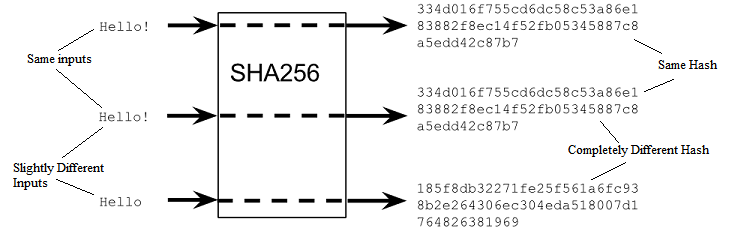
\includegraphics[scale=0.7]{pics/BlockOverviewSHA.png}
\end{figure}
\vspace{10mm}

\begin{itemize}
    \item The nonce value is chosen arbitrarily at first, and then inserted into the header.
    \item The header of the block is then converted into 160 character string.
    \item The hash of this header is computed using the SHA-256 algorithm, and the final 32 character result is compared to the \textit{target}
    \item The target is a 32 character string chosen by the network with a set amount of zeros in the beginning. The more the number of zeros, the harder it is to solve the mining problem.
    \item As mining requires one to compare the hash of the block header such that it is lesser than the target, anyone that wins this should either be really lucky, or have enough computational power to run through more than $10^{15}$ hashes per second or so. 
    
\end{itemize}
\vspace{10mm}

Being capable of running SHA-256 so many times in a second is more of a reliable method to get the block hash lesser than the target, and so miners rely on their hardware capabilities than just luck. \newline

For example, if the target value of a block is set to the number $100$, then the total possible hashes that are allowed would range from $[0,100]$. Since the SHA-256 outputs a $256$ bit number, the total probability that a single node gets a hash right would be $\dfrac{100}{2^{256}-1}$ which is almost zero, practically.\newline
If the target were to be set to something like say, $2^{128}$, then the total number of guesses drastically rises and so the probability that a node gets a hash lesser than $2^{128}$ would be approximately $\dfrac{1}{2^{128}}$  .

\vspace{10mm}
The bitcoin network constantly adjusts the value of this target so that on an average, the network only mines one block every 10 minutes. Notice that since more than one node is trying to guess the nonce for a hash, lesser than the specified target, the probability that at least one node gets it right is much much higher than just one node trying it out.

\vspace{10mm}
\textbf{7.3 TRANSACTIONS}
\vspace{7mm}

Now let us take a closer look into the actual structure of transactions that occur on the bitcoin network. A transaction can be taught of as a system with multiple inputs and multiple outputs.\newline
To further understand this system, let us look at the steps the network takes to send money to another account, from the current one.\newline
A sender of Bitcoins, in the current transaction firstly signs that they are indeed authorising the movement of funds. Only when this check is done would the transaction proceed further. The sender's hashed private key is sent along with the public key, to verify. Once verified, the sender \textit{puts in bitcoins greater than or equal to the amount they want to spend,} along with the intended recipient's public key as the address of the wallet. Next the funds to be transferred is written in the output of this transaction. If any coins are left over as change, there will be another output created in this transaction, referring to the original owner of the bitcoins as the intended recipient and they would receive the change.\newline



\begin{figure}[h]
\centering
\caption{Multiple Input and Multiple Output Transaction Structure}
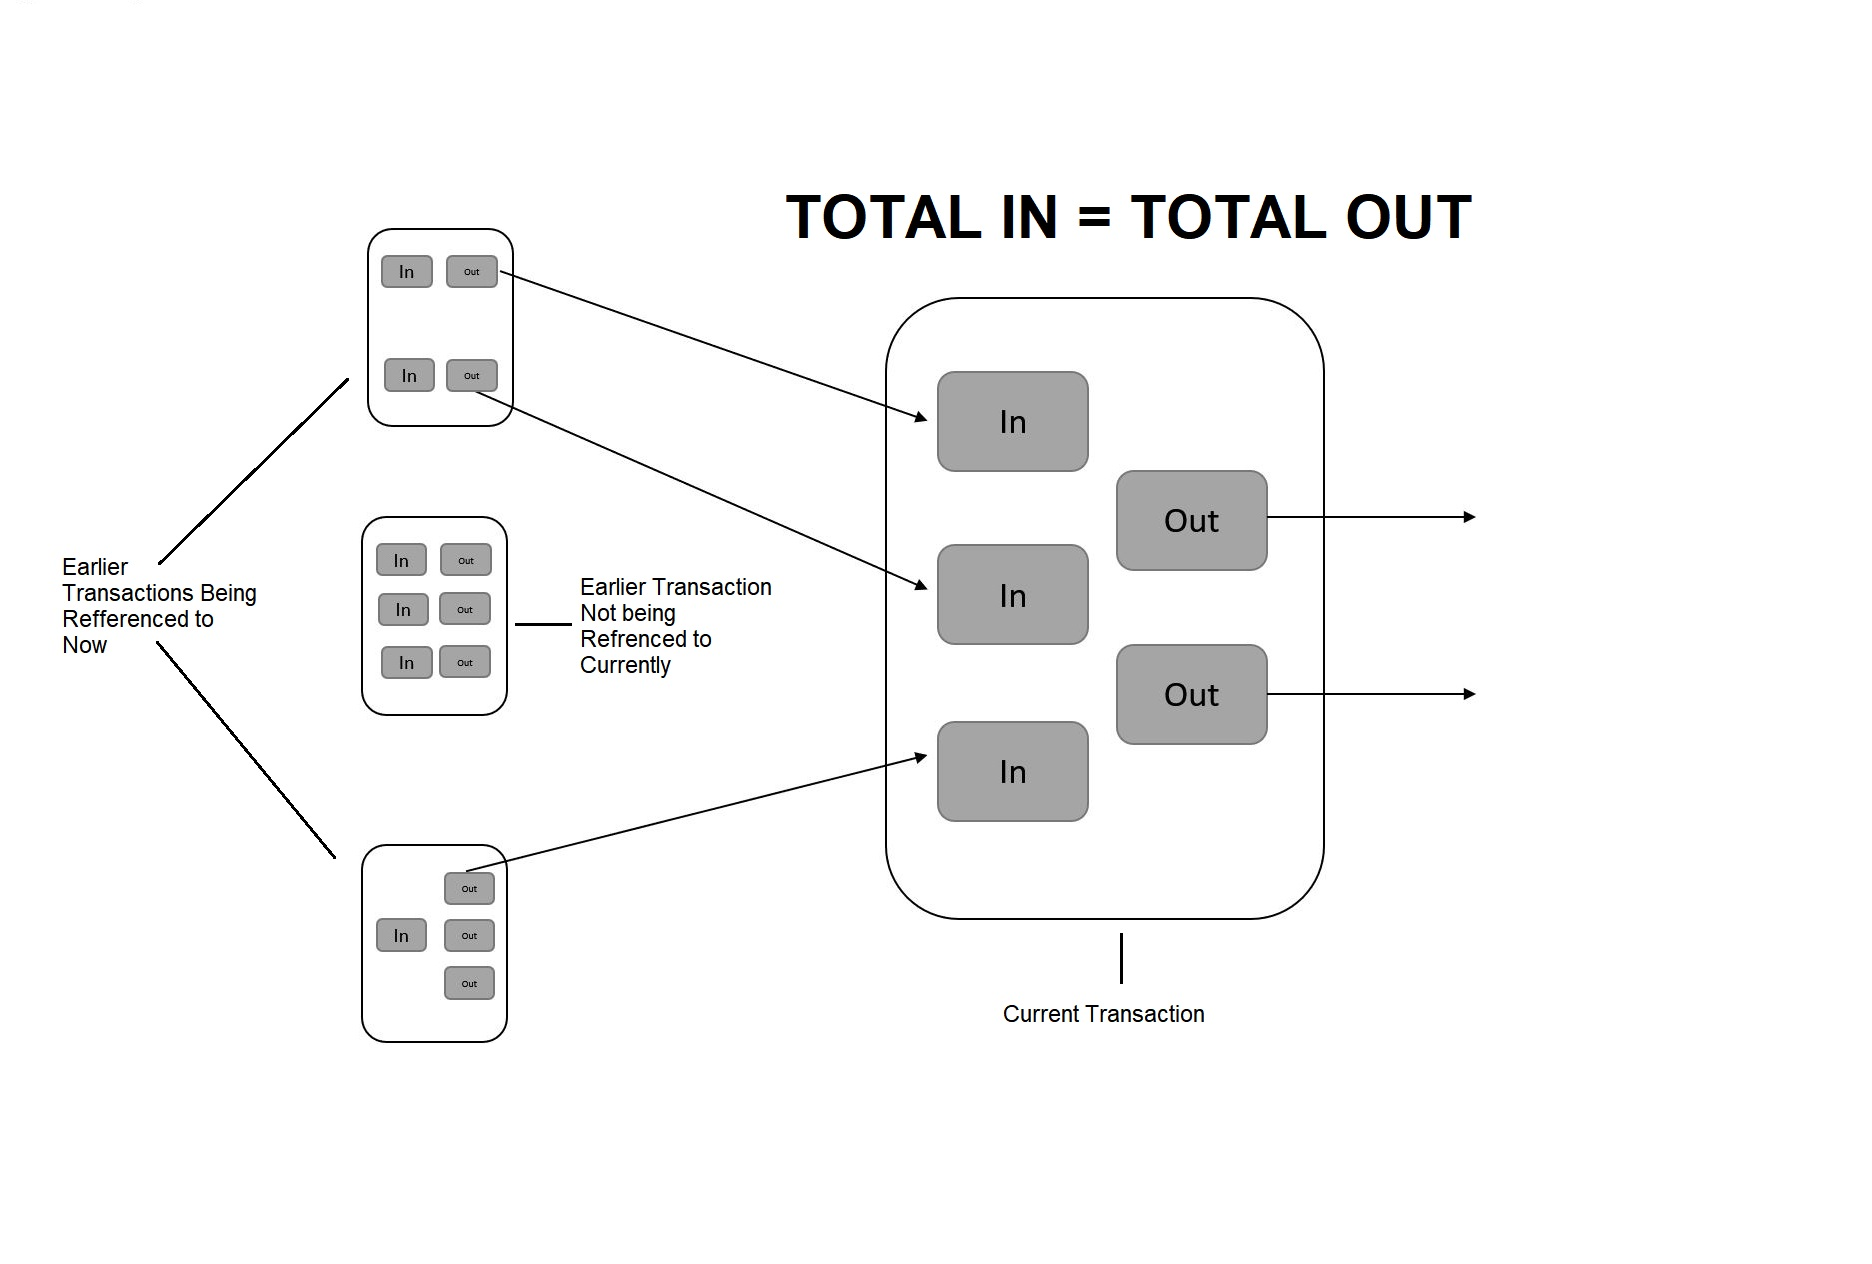
\includegraphics[scale=0.4]{pics/Transac.JPG}
\end{figure}

This way, transactions would not need a serial number as every single transaction just contains references to outputs of previous transactions as its inputs. Any of the mentioned recipients in the current transaction can then just refer to the output of this, if they would wish to \text{spend} the bitcoins they got from this transaction.\newline
Note that in the bitcoin network, transaction outputs can be refereed to only once. The change received from any transaction acts as a new input to the owner of those coins. Thus to tally up someone's bitcoin wallet would be to add all the unreferenced outputs of various transactions, that have that public key as the recipient address which is associated to the private key of the holder of the said bitcoins. This is what is meant to \textit{own} bitcoins. 
\vspace{10mm}

Now, the very first block that was created had no inputs to refer to, and this was an exception. Also, if one traverses back through transactions, they would end up wither at the first ever block, the \textit{genesis block}, or more likely, reach a \textit{coinbase}. A coinbase reward is a transaction written on every block that has no source, but is just created out of thin air. It is awarded to the miner of a block. This \textit{reward} is a block reward, and it halves for every 2016 blocks that are added onto the chain. The genesis block had a reward of 50 bitcoins and had only that as the transaction in it. Thus, it can be shown that if we add up this converging series of block rewards, the total number of bitcoins that would ever be in circulation will be 21 million. No more, or no less.

\newpage

\begin{center}\underline{ \Large \textbf{CHAPTER 8}}\end{center}
\begin{center}\underline{ \Large \textbf{THE CAVEATS}}\end{center}
\vspace{10mm}

The bitcoin network may be very cleverly designed, but it is not without its shortcomings. This network does have a few problems, which is why newer cryptocurrencies are slowly gaining traction. The demerits could be summarised as follows: 
\begin{itemize}
    \item The network has very long processing times. Since a block gets added every minute, people have to wait for transactions to get confirmed. Also, just because a transaction is added to the blockchain doesn't guarantee that it is confirmed. This is because of forks.
    \item A fork in the blockchain refers to having two or more blocks, with different header hashes, having the same previous hash field in it. This could mean that two or more nodes coincidentally mined the same block, and put it on the blockchain before everyone else on the block knew about it.\newline
    Because of this, some would follow one path on the chain, and others, another. The actual main blockchain would, however, be the \textit{longest} one, in terms of computational power. This means that if one of the fork is chosen as the main path, it would be because nodes that built on it, have done the most work on it.
    \item The anonymity bitcoin provides leads to it being used in black markets and has the potential to be used to finance a lot of illegal activities since it is an untraceable currency.
    \item If a transaction is lost, by some freak accident, then there is nobody to help return it. There isn't any customer support that is provided, and so people would just end up losing the bitcoins.
    \item Bitcoin remains susceptible to wild price swings over short periods of time. In the wake of the Mt. Gox collapse, Bitcoin’s value fell by more than 50\%. Following the FBI’s announcement that it would treat Bitcoin and other virtual currencies as “legitimate financial services,” Bitcoin’s value spiked by a similar amount. While Bitcoin’s volatility sometimes offers short-term benefits for speculative traders, it renders the currency unsuitable for longer-term investors.
\end{itemize}



\newpage
\begin{center}\underline{ \Large \textbf{CONCLUSION}}\end{center}
\vspace{10mm}
This paper has summarised the inner workings of the bitcoin network and currency system. It was shown to be an electronic transaction system that doesn't rely on  trust, but computer science and cryptography. We started of with the motivation behind the creation of bitcoins, and after dwelling in some history and facts, we went right into the challenges faced by any cryptocurrency.\newline
We showed that digital currencies can provide a strong control of ownership, but is just one of the few things needed to build a complete cryptographic currency system.
The double spending issue was also mitigated and we also showed how the network is Byzantine Fault Tolerant. This was done by introducing the Proof-of-Work, which eliminates any trust, and mitigates the fault.\newline
This Proof-of-Work was shown to be nothing but a mere way of guessing the input to the SHA-256 hashing algorithm (which was also briefly explained) such that the hash would lie below a certain target threshold.
The network is robust in its unstructured simplicity. Nodes work all at once with little coordination, without the need to be identified.\newline
The disadvantages of bitcoins was also looked into and the blockchain was explained along with the various fields of the block. The Merkle Root, the block hash, the Version field, the Bits field, the Nonce and the time-stamp. An actual bitcoin transaction was also looked into and the true meaning of owning a bitcoin was shown to be just the addition of \textit{all the unreferenced outputs of various transactions, that have that public key as the recipient address which is associated to the private key of the holder of the said bitcoins.}\newline

\newpage
\begin{center}\underline{ \Large \textbf{REFERENCES}}\end{center}

[1] S. Nakamoto. Bitcoin: A peer-to-peer electronic cash system. www.bitcoin.org.\\

[2] Courtois, N. T., Grajek, M., & Naik, R. (2013). The Unreasonable Fundamental Incertitudes Behind Bitcoin Mining. arXiv preprint arXiv:1310.7935.\\

[3] Babaioff, M., Dobzinski, S., Oren, S., & Zohar, A. (2012, June). On bitcoin and red balloons.
In Proceedings of the 13th ACM Conference on Electronic Commerce (pp. 56-73). ACM.\\

[4]https://medium.com/@micheledaliessi/how-does-the-blockchain-work-98c8cd01d2ae\\

[5] http://www.michaelnielsen.org/ddi/how-the-bitcoin-protocol-actually-works/\\

[6] https://www.youtube.com/watch?v=UZBZPOEVyJA\\

[7] https://www.youtube.com/watch?v=gUwXCt1qkBU






\end{flushleft}



\end{document}

